
%%%%%%%%%%%%%%%%%%%%%%%%%%%%%%%%%%%%%%%%%%%%%%%%%%%%%%%%%%%%%%%%%%%%%%%%%%%
%%% MOTIVATING EXAMPLE
%% \newcommand{\nilfigure}
%% {\scalebox{0.75}{
%% \psset{unit=1mm,nodesep=0mm,labelsep=0.5mm}
%% \begin{pspicture}(0,0)(1,1)
%% %\psgrid[xunit=1cm,yunit=1cm,gridwidth=.2pt,subgridwidth=.1pt,subgriddiv=5,subgridcolor=gray,gridcolor=blue](0,0)(1,1)
%% \putnode{start}{origin}{0}{0}{}
%% \putnode{stop}{origin}{10}{10}{}
%% \ncline[offsetB=0,nodesepB=0,linewidth=.7]{-}{start}{stop} %here
%% \end{pspicture}
%% }}

%\begin{columns}
 % \begin{column}{0.5\textwidth}
%\begin{boxedminipage}{\textwidth}{
    \scalebox{0.75}{\sf
      \renewcommand{\arraystretch}{1}{
	\begin{uprogram}
	  \UFL\ \hspace*{-.31\TAL} (\DEFINE\ (\plength\  \lista)
	  \UNL{1}  (\SIF~(\NULLQ \ \lista)
	  0
	  \UNL{2}      ($+$\ 1\ (\plength\ (\CDR\  \lista)))))
          \UNL{2}
          \UNL{0}\ \hspace*{-.31\TAL} (\DEFINE\ (\pfun\  \listb)
	  \UNL{1}  ($+$\ 1\ (\CAR\  \listb)))
          %         \UNL{2}\;\;\;\;\;
          \UNL{0}
	  \UNL{0} \hspace*{-.49\TAL} $\pi_\mainpgm$ : (\LET\ \pz\   $\leftarrow$(\CONS\ ($+$\ $4$ $5$)\
          \UNL{0} \;\;\;\;\;\;\;\;\;\;\;\;\;\;\;\;\;\;\;\;\;\;\; (\CONS\ ($+$\ $5$ $2$) \NIL)) \IN
	  \UNL{0} \;\;\;\;\;\;\;\;\;\;\;\;(\SIF\ $*$\ 
	  \UNL{1} \;\;\;\;\;\;\;\;\;\;\;\; $\pi_1$: (\plength\ \pz\ )
	  \UNL{1} \;\;\;\;\;\;\;\;\;\;\;\; $\pi_2$: (\pfun\ \pz\ )))
	\end{uprogram}
  }}
%\end{boxedminipage}
  %% \end{column}
  %% \begin{column}{0.5\textwidth}
  %%   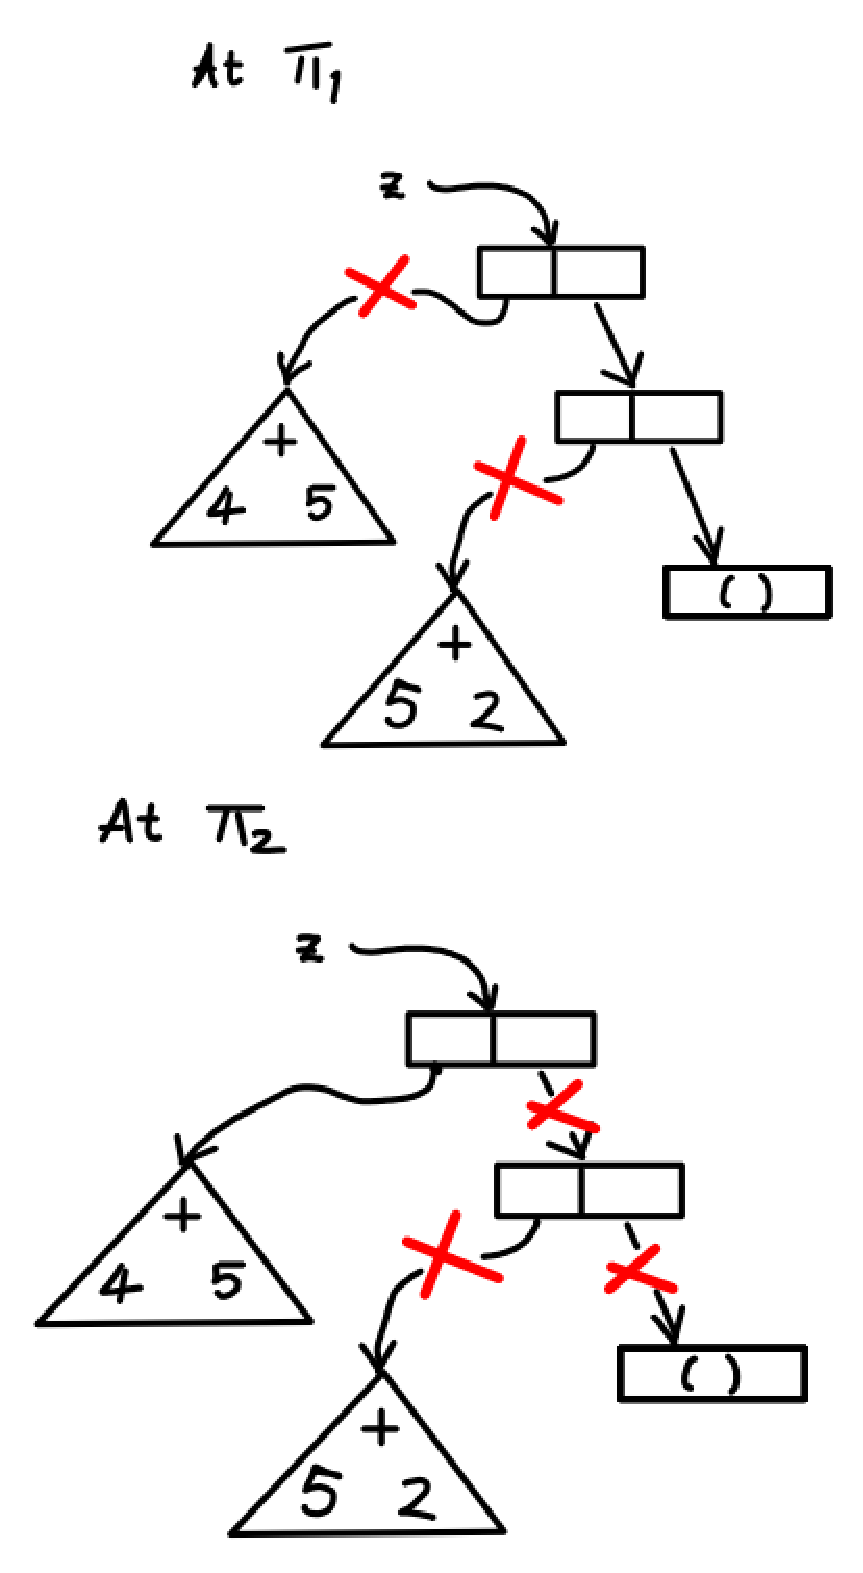
\epsfig{file=mem-graph.eps, height=6.5cm}
  %% \end{column}
%\end{columns}

